\chapter{ミュージックステーシオン}
\section{概念歌feat.琉球乃笑}

\subsection{歌詞}

目を閉じれば 億千のグバ\\
 一番光る オバがいる
\section{ズンドコ津与志}
\subsection{歌詞}
勝手にふられて 華が咲く\\
勝手にふられて 華が咲く\\
男ならでは 旅に出て\\
ああ日本海 美しい\\
ズン ズンズン ズンドコ きよし\\
ズン ズンズン ズンドコ きよし\\
\\
糧に振られて 鼻が割く\\
糧に振られて 鼻が割く\\
無駄に振られて 酒蔵へ\\
ああ今宵は 酒祭り\\
ズン ズンズン ズンドコ きよし\\
ズン ズンズン ズンドコ きよし\\

\newpage
\section{がんばれ、みんな}
\subsection{歌詞}
\ \\ 
オオオオオー\\
\\
ダメだった\\
うまくいかない\\
そんなことばかりよね\\
\\
それでもね\\
進んでいくの\\
ちゃんと前を向いて\\
\\
間違えることでやっと\\
わかることだってあるかな\\
あきらめないでいこう\\
どんなことがあったとしても\\
何度でも ダメだったとしても\\
向かっていけばいいよ\\
\\
あきらめないでいこう\\
どんなことがあったとしても\\
何度でも そう何度だって\\
向かっていけばいいよ\\
\\
あきらめないでいこう\\
どんなことがあったとしても\\
何度でも \ そう何度だって\\
向かっていけばいいよ\\
 \\
オオオオオー\\
やるのよ\\
オオオオオー\\
何度も\\
オオオオオー\\
やるのよ\\
オオオオオー\\

\section{クソの極みおちんぽこ}
\subsection{リリース曲}
 \\
1.言っとくけど奢らんぞ\\
2.いいよ(仮)\\
3.上原は今、隠れん坊をしております\\
4.万年南/平社員\\
5.それはほざいてるfeat.お山インティライミ\\

%\pbox<t>{aaa}
\newpage
\section{ファー ファファッファファファファファー}
学部生時代にLANS BOXで昼食を取っていたときに、食堂内にオルゴールver.に編曲されているJ-POPが流れていた。知っている曲が多数を占める中、唯1曲だけタイトルが分からず、ボーカルの声・グループも全く分からない曲が流れた。しかし、私は聞き覚えがあったのだがそのメロディを口ずさんで友人に聞かせてみても「聞いたことあるが、分からない、、、。」との答えが返ってくるのみ。この時からこの曲が何なのかという問題が生じ、約3年間に渡って物理家を悩ませることとなった。\par
それは2016年12月28日のことである。
\begin{figure}[h]
  \centering
  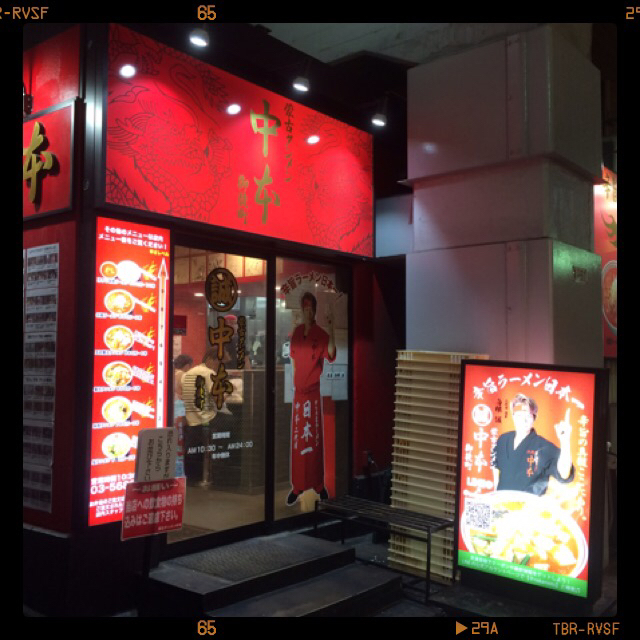
\includegraphics[width=7cm]{mouko_tanmen.jpg}
  \caption[]{JR御徒町駅周辺にある素晴らしいラーメン店}
  \label{fig_hoge1}
\end{figure}
舞台は図\ref{fig_hoge2}に見るラーメン店であった。\\私と友人は激辛ラーメンを求めてこのラーメン店を訪れた。そして友人は味噌タンメン(辛さ1)を、私は北極ラーメン(辛さ9)を注文した
\footnote{このスープをレンゲで頂いた時に盛大に咽てしまったのはまた別の話である。}。
\begin{figure}[h]
  \centering
  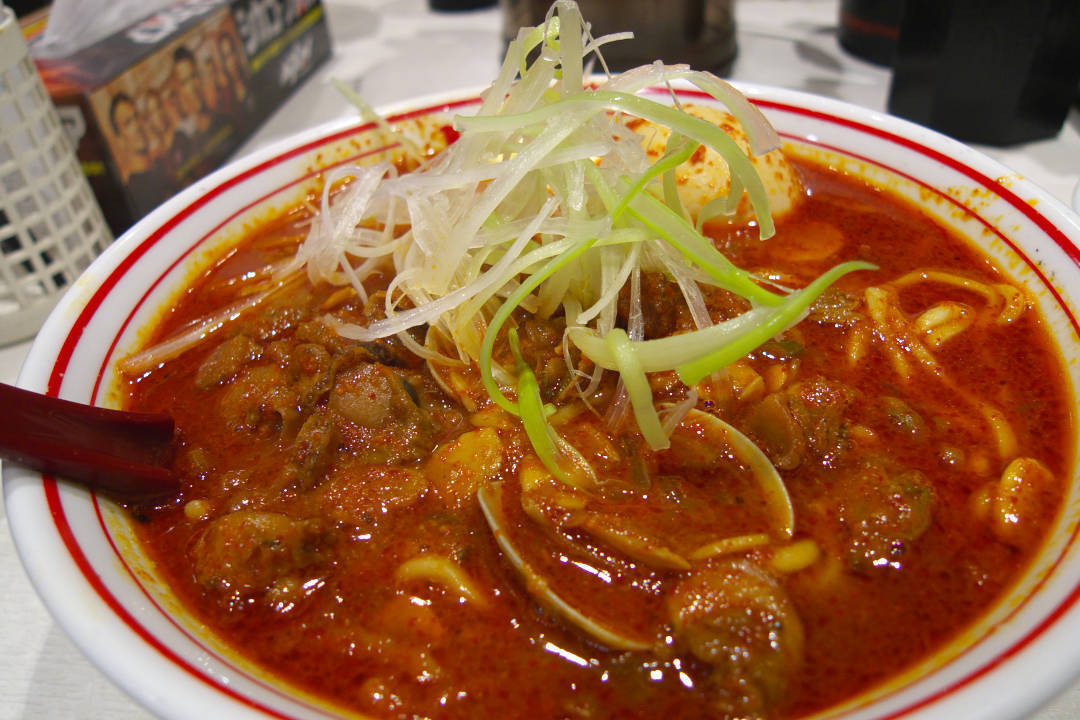
\includegraphics[width=7cm]{hokkyoku.jpg}
  \caption[]{辛さ9の北極ラーメン}
  \label{fig_hoge2}
\end{figure}
汗だくになりながら食べている時に、ふと店内に流れているBGMが耳に飛び込んできた。その時に私は飛べるのを止め、咄嗟にGoogleChromeを起動して店内のBGMの歌詞を聞き取り「愛してる言葉の意味を」と検索窓に叩き込んだ。そして出てきた検索結果が全世界の物理屋を驚愕させた。\\
\begin{center}
アイシテル/monkey majik
\end{center}
%%%%%%%%%%%%%%%%%%%%%%%%%%%%%
